\chapter{Result}\label{ch:result}
\section{Model verification}
The model presented in chapter \ref{ch:designing_and_modeling} was verified
with the verification queries presented in the same chapter.

\begin{itemize}
    \item For deadlock verification the property was satisfied.
    \item For livelock verification the property was not satisfied.
\end{itemize}

% \section{Time-triggred and event-triggered systems}
% TODO: Write down the different results I found (the properties/attributes to be
% measured must be defined in the problem statement).

\section{Implementation}
The implemented SPA framework code called "Virtual Network Library" is
available on Github at \url{https://github.com/virtualnetwork/vn-lib}
(including the third iteration and final UPPAAL model). The
modular design is shown in figure \ref{fig:appendix_component_overview} and the
source code compiles with the Ravenscar restrictions. Efforts have also been
made to limit the amount of dynamic memory usage.

Example implementation is available in the "examples" directory in the git
repository. Below is a series of images that show example output from a test
run. The example output is the same process as is described in section
\ref{sec:discovery_process} with UML sequence diagrams.

\begin{figure}[ht]
    \centering
    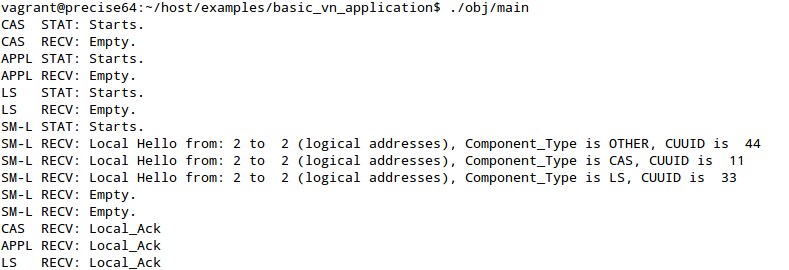
\includegraphics[width=\textwidth]{figures/code_part_1}
    \caption{First the configured components start and send out Local\_Hello
    messages which are processed by the SM-L. SM-L replies with Local\_Ack to
    all other components and a specific Request\_Address\_Block to the CAS.}
    \label{fig:code_part_1}
\end{figure}

\begin{figure}[ht]
    \centering
    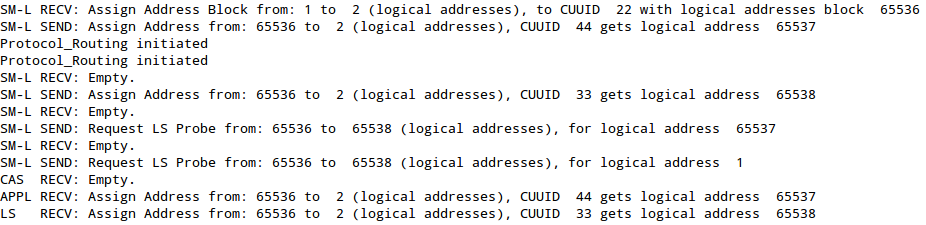
\includegraphics[width=\textwidth]{figures/code_part_2}
    \caption{The CAS replies with Assign\_Address\_Block which is processed by
    the receiving SM-L. After this the SM-L starts to hand out logical
addresses to all components in the local interconnect. The logical addresses
are received by all applications. As a last step the SM-L sends out
Request\_LS\_Probe messages to the LS for all components on the local
interconnect. This last step is the end of the network discovery process and
the start of the component data capabilities discovery process.}
    \label{fig:code_part_2}
\end{figure}
